% More specifically, using spike sorted data recorded from the mouse brain stem in the pedunculopontine and laterodorsal tegmental (PPT/LDT) areas, we address whether these areas do in fact initiate sleep stages, which has been previously hypothesised and recently debated. 
% To address this, we looked at the temporal relationship between future and past state prediction, using linear discriminant analysis (LDA) on derived functional modules using non-negative matrix factorisation (NMF), replicating and extending the work reported by the collaborative lab from whom we have been granted access to the spike data.
% Further, we study methodologies for inferring meaningful computational models using spike train data, and how they inferred models may be studied to evaluate the nature of the neurons by drawing upon the biology corresponding to their parameters within the literature.
% This algorithmic approach applied to spike train data has, to the best of my knowledge, not been previously explored. This is due to the high dimensional parameter search space, which requires a correspondingly complex approach in order to make computation tractable.
% As such, not only could an inferred model be used to address hypotheses such as whether sleep regulation within this area is mediated by an ensemble of cholinergic neurons, but the methodology could further be applied in other domains, using data of the same nature from different brain regions.
% The approach requires only partial data - as is always a constraint within neuroscientific recordings. 
% Using a form of Bayesian inference, measures of deviation and confidence may be defined comparatively between synthetic models and data, and the recorded spike trains considered as ‘ground truth’. Probable fits with a fair variance suggest meaningful inferred model parameter distributions. However, model quality metrics depend on the data for which the comparison is computed.

% More specifically, the model inference method is based on modelling the probability of spiking for a neuron as a Bernoulli random variable, with the variable modelling spiking in each time bin. We construct time bins for the spike trains such that the probability of spiking in one bin may be approximately dependent only on the previous bin (which might be justified considering its refractory and synaptic time constants). This allows us to formulate the probability of a spike train as a Markov chain, and enables us to estimate population model parameters. Interestingly, the authors found that a better fit for a microscopic model was inferred when first performing gradient descent for a mesoscopic level model, representing each population with average parameters. 
% This may be due to that inferring only one average parameter value per population regularises the training procedure by averaging over the parameter space of a microscopic model. 
% There are two key points that I would like to communicate associated with that observation; (1) is that the complexity associated with the parameter space of microscopic models might make convergence towards a global optimum unlikely, and (2) that an average parameter might lose values that are of a secondary or tertiary order of importance, despite prominent in the data set, if somewhat conflicting with the final inferred average value. Addressing (2), it might be fruitful to allow for sets of average values for population models, investigating whether this might increase resulting microscopic model performance. Note that inference of the maximum a posteriori for corresponding microscopic models then might increase exponentially, or at least linearly, with the order of increased number of values inferred at the mesoscopic level. However, it might make sense to infer one average per neuron type as the population level, i.e. if it is believed that it contains for instance two sets of neuron types, or functional ensembles, such as inhibitory-excitatory neurons. This has to my knowledge not been attempted within this methodological approach.
% Once a mesoscopic model has been attained, it may be used to synthetically generate data for use in the inference of a more detailed neuron-level or microscopic model. By generating synthetic data we may employ the family of Monte-Carlo (MC) methods. In order to accelerate convergence for computational efficiency, Hamiltonian MC is employed. This allows for approximating the full posterior over the most likely parameter distributions for microscopic models.

% Statistically, model soundness may be considered in terms of comparison to a validation set stemming from the same experiment, and also across the 7 performed experiments. However, due to the nature of neuroscientific recordings, where there is a significant uncertainty in both the areas targeted with the silicon probes, and not the least due to significant individual differences for neural ensembles, it is unlikely that we can see neuron-level similarities across experiments. However, similarities at a population and functional level may occur if the same areas are recorded.



%  for \textbf{GBO (top)} and \textbf{SBI (bottom)}.
% SBI
% \begin{figure}
%     \centering
% 	\includegraphics[width=0.49\columnwidth]{figures/}
% 	\includegraphics[width=0.49\columnwidth]{figures/}
% 	\caption{Fitted model rates across model types and loss metrics, and average parameter distance between the ground-truth model and both the initial and converged inferred models for GBO (top) and SBI (bottom).}
% \end{figure}

%sample microGIF poisson & bernoulli
% export_microGIF_plot_loss_euid_12-09_16-36-58-996.eps
% export_param_inference_X_microGIF_1_E_L_.eps
% export_spike_trains_euid_12-09_16-36-58-996.eps


% BIN_SIZE = 1/9
% massive_dict keys: dict_keys(['correlations_OU_per_model_type', 'activity_rmse_OU_per_model_type', 'correlations_wn_per_model_type', 'activity_rmse_wn_per_model_type', 'correlations_OU_per_model_type_per_pop', 'activity_rmse_OU_per_model_type_per_pop', 'correlations_wn_per_model_type_per_pop', 'activity_rmse_wn_per_model_type_per_pop'])
% correlations_OU_per_model_type_per_pop BNLL [[0.136229   0.45113911]
%  [0.16280599 0.28163129]
%  [0.07925058 0.45339818]
%  [0.08042286 0.51556134]]
% activity_rmse_OU_per_model_type_per_pop BNLL [ 8.741314 10.78977  16.814838 28.585888]
% correlations_wn_per_model_type_per_pop BNLL [[-0.04303113  0.48399174]
%  [-0.05307253  0.47993182]
%  [ 0.09430935  0.54154142]
%  [-0.13191614  0.4481658 ]]
% activity_rmse_wn_per_model_type_per_pop BNLL [ 8.9276905 11.528968  19.901028  29.041882 ]
% correlations_OU_per_model_type_per_pop PNLL [[ 0.21973303  0.39076739]
%  [-0.03306306  0.48793001]
%  [ 0.03666054  0.65488266]
%  [ 0.03208419  0.47790354]]
% activity_rmse_OU_per_model_type_per_pop PNLL [11.170116 13.295268 17.302729 25.481037]
% correlations_wn_per_model_type_per_pop PNLL [[-0.03063577  0.59096444]
%  [ 0.09773039  0.48791501]
%  [-0.0160414   0.44861028]
%  [ 0.0196374   0.62583975]]
% activity_rmse_wn_per_model_type_per_pop PNLL [11.527083  14.5694475 19.83553   25.033321 ]


% ==================== ----------------------- 16.01.2022 ==================== ----------------------
% *** https://docs.scipy.org/doc/scipy/reference/generated/scipy.stats.pearsonr.html

% massive_dict keys: dict_keys(['correlations_OU_per_model_type', 'activity_rmse_OU_per_model_type', 'correlations_wn_per_model_type', 'activity_rmse_wn_per_model_type', 'correlations_OU_per_model_type_per_pop', 'activity_rmse_OU_per_model_type_per_pop', 'correlations_wn_per_model_type_per_pop', 'activity_rmse_wn_per_model_type_per_pop'])
% correlations_OU_per_model_type_per_pop BNLL unfiltered mean: [[0.136229   0.45113911]
%  [0.16280599 0.28163129]
%  [0.07925058 0.45339818]
%  [0.08042286 0.51556134]]
% num "converged": 14
% correlations_OU_per_model_type_per_pop BNLL filtered w threshold: 0.2 [[0.2285608  0.45060827]
%  [0.35417916 0.29010902]
%  [0.13811508 0.46374777]
%  [0.13586292 0.53474661]]
% correlations_wn_per_model_type_per_pop BNLL unfiltered mean: [[-0.04303113  0.48399174]
%  [-0.05307253  0.47993182]
%  [ 0.09430935  0.54154142]
%  [-0.13191614  0.4481658 ]]
% num "converged": 10
% correlations_wn_per_model_type_per_pop BNLL filtered w threshold: 0.2 [[0.09267896 0.60143853]
%  [0.14028457 0.58431124]
%  [0.20588619 0.55422147]
%  [0.07390235 0.49125028]]
% correlations_wn_per_model_type_per_pop PNLL unfiltered mean: [[ 0.21973303  0.39076739]
%  [-0.03306306  0.48793001]
%  [ 0.03666054  0.65488266]
%  [ 0.03208419  0.47790354]]
% num "converged": 16
% correlations_wn_per_model_type_per_pop PNLL filtered w threshold: 0.2 [[ 0.26594066  0.43419887]
%  [-0.01944962  0.59813733]
%  [-0.0220576   0.68623279]
%  [ 0.03665507  0.52298418]]
% correlations_wn_per_model_type_per_pop PNLL unfiltered mean: [[-0.03063577  0.59096444]
%  [ 0.09773039  0.48791501]
%  [-0.0160414   0.44861028]
%  [ 0.0196374   0.62583975]]
% num "converged": 17
% correlations_wn_per_model_type_per_pop PNLL filtered w threshold: 0.2 [[0.0135526  0.61893445]
%  [0.0820617  0.46132494]
%  [0.05597967 0.48230394]
%  [0.05354188 0.68179549]]
% activity_rmse_OU_per_model_type_per_pop BNLL [ 8.741314 10.78977  16.814838 28.585888]
% activity_rmse_wn_per_model_type_per_pop BNLL [ 8.9276905 11.528968  19.901028  29.041882 ]
% activity_rmse_OU_per_model_type_per_pop PNLL [11.170116 13.295268 17.302729 25.481037]
% activity_rmse_wn_per_model_type_per_pop PNLL [11.527083  14.5694475 19.83553   25.033321 ]

% table
% init_rmse_wn [array(15.597686, dtype=float32)]
% rmse_wn [29.394892]
% init_rmse_OU [array(3., dtype=float32)]
% rmse_OU [29.588663]
% n_init_rmse_wn tensor([1.])
% n_rmse_wn tensor([1.8846])
% n_init_rmse_OU tensor([1.])
% n_rmse_OU tensor([9.8629])
% init_corrs_wn [array(1.5, dtype=float32)]
% correlations_wn [0.1]
% init_corrs_OU [array(3., dtype=float32)]
% correlations_OU [-0.19999999]

% init_rmse_wn [array(12.2687, dtype=float32)]
% rmse_wn [26.907501]
% init_rmse_OU [array(0., dtype=float32)]
% rmse_OU [26.815296]
% n_init_rmse_wn tensor([1.])
% n_rmse_wn tensor([2.1932])
% n_init_rmse_OU tensor([nan])
% n_rmse_OU tensor([inf])
% init_corrs_wn [array(-0.5, dtype=float32)]
% correlations_wn [0.16666667]
% init_corrs_OU [array(0., dtype=float32)]
% correlations_OU [1.1920929e-08]

% GBO
% init_rmse_wn [array(14.968042, dtype=float32)]
% rmse_wn [12.033964]
% init_rmse_OU [array(2., dtype=float32)]
% rmse_OU [11.603041]
% n_init_rmse_wn tensor([1.])
% n_rmse_wn tensor([0.8040])
% n_init_rmse_OU tensor([1.])
% n_rmse_OU tensor([5.8015])
% init_corrs_wn [array(1., dtype=float32)]
% correlations_wn [0.25]
% init_corrs_OU [array(2., dtype=float32)]
% correlations_OU [-0.125]

% np.mean(correlations_OU_per_model_type_per_pop['microGIF'], axis=0)
% Out[9]: 
% array([[ 0.04449298,  0.53082549],
%       [ 0.03504001,  0.50368762],
%       [-0.04568029,  0.53626128],
%       [-0.01166335,  0.52908753]])
% np.mean(correlations_wn_per_model_type_per_pop['microGIF'], axis=0)
% Out[10]: 
% array([[ 0.06472507,  0.56145749],
%       [ 0.12279707,  0.41758472],
%       [-0.01644223,  0.46314913],
%       [ 0.20302207,  0.40018902]])

% np.mean(activity_rmse_wn_per_model_type_per_pop['microGIF'], axis=0)
% Out[11]: array([29.468164, 38.342987, 58.59618 , 79.747246], dtype=float32)
% np.mean(activity_rmse_OU_per_model_type_per_pop['microGIF'], axis=0)
% Out[12]: array([28.68748 , 35.648613, 49.524837, 80.788055], dtype=float32)

% correlations_OU_per_model_type_per_pop BNLL [[ 0.03672772  0.54079383]
%  [ 0.03348813  0.56219029]
%  [-0.07295515  0.48390601]
%  [ 0.02472201  0.62395228]]
% activity_rmse_OU_per_model_type_per_pop BNLL [24.281664 31.598572 48.442345 85.50205 ]
% correlations_wn_per_model_type_per_pop BNLL [[ 0.06963954  0.54004642]
%  [-0.15062001  0.37560239]
%  [ 0.32837038  0.56875123]
%  [ 0.28102542  0.41184876]]
% activity_rmse_wn_per_model_type_per_pop BNLL [25.138638 33.444435 58.565758 85.78223 ]
% correlations_OU_per_model_type_per_pop PNLL [[ 0.05225825  0.52085716]
%  [ 0.03659189  0.44518495]
%  [-0.01840543  0.58861656]
%  [-0.04804871  0.43422278]]
% activity_rmse_OU_per_model_type_per_pop PNLL [33.0933   39.69866  50.607323 76.07405 ]
% correlations_wn_per_model_type_per_pop PNLL [[ 0.05981061  0.58286855]
%  [ 0.39621414  0.45956705]
%  [-0.36125484  0.35754704]
%  [ 0.12501872  0.38852927]]
% activity_rmse_wn_per_model_type_per_pop PNLL [33.797703 43.241554 58.6266   73.71228 ]



% General description across p-dists, and mostly rates (implicitly loss).

% \begin{figure}
% 	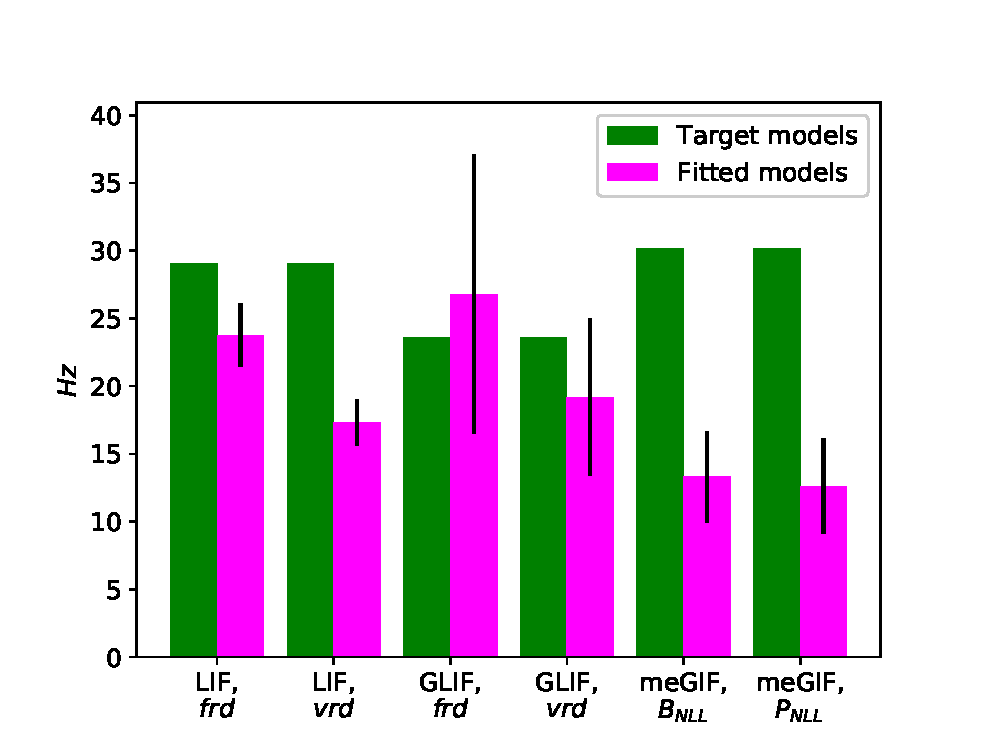
\includegraphics{figures/export_rates_only_GT_all.eps}
% \end{figure}

% bugged_mesoGIF_4.eps
% bugged_microGIF_4.eps
% bugged_microGIF_21.eps
% export_GLM_filters_pred_bin_size_0_1_cell_2_target_GT_model_GLIF_N_4.eps
% export_GLM_filters_pred_bin_size_0_1_cell_2_target_GT_model_LIF_N_4.eps
% export_GLM_filters_pred_bin_size_0_1_cell_2_target_GT_model_mesoGIF_N_4.eps
% export_GLM_filters_pred_bin_size_0_1_cell_2_target_GT_model_microGIF_N_21.eps
% geodesic_distances_Synthetic_GLIF.eps
% geodesic_distances_Synthetic_LIF.eps


% =============== roughly chpt 4 ===============

\subsection{Shared synthetic data set across model types}
Fitting to the same synthetic data set, such that we may compare performance across model types for the same data set. 
This data was generated by a hand-engineered ...

\begin{figure}
    \centering
	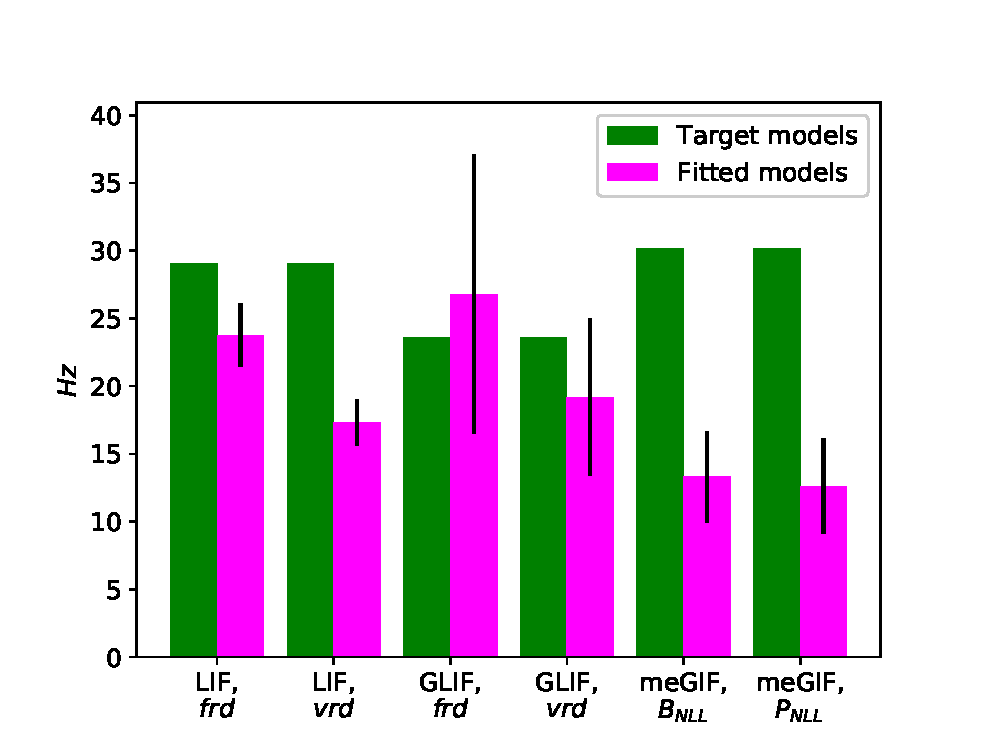
\includegraphics[width=0.49\columnwidth]{figures/export_rates_only_GT_all.eps}
\end{figure}

% \begin{figure}
% 	\includegraphics{figures/}
% \end{figure}


% \subsection{Leaky integrate-and-fire (LIF)}

% Gradient-based methods prone to finding sub-optimal solutions, i.e. local minimas. This is an issue particularly for high-dimensional feature spaces. Thus, I am led to believe this will be an issue when trying to infer the model parameters of complex neural networks using spike trains.

% %--------------------
% LIF work log:
% More nuanced
% Very noisy gradients for unstable/chaotic generative model perturbation?
% Dynamic R\_I in conjunction with frd might result in better convergence, due to constraining search space.
% By using dynamic R\_I (linear constraint), this makes behaviour more stable, and so may allow for more calibration/optimisation of the other parameters.

% % vRD suddenly seems viable for more stable network behaviour. When model behaviour was more chaotic, frd was better. This makes sense, as gradient will not be well-defined for vRD when model is chaotic. Not necessarily for frd either, but this is more robust to noise.

% Some artefacts LIF (more linear, easier to have whole-network spiking with too little inhibition / simpler neuron dynamics)

% Initial conditions large effect on convergence

% vRD performance OK with tau=100.0
% frd better
% In conjunction: still sometimes silent neurons. Potentially due to local minima of vRD for silent neurons, and obscured parameter-landscape due to noise and the nature of the vRD-metric. Not necessarily orthogonal to frd either, and as such may interfere with its gradient

% Will have to look at vRD vs frd vs frd+vRD vs adaptive(frd+vRD) quantitatively for setups.

% There seem to be many regions for which there is no “information gain” when moving along gradients, such as for silent neurons. Some parameters might not have their effect obscured or less pronounced due to the change of other parameters in parallel, too. This is the reason other authors have performed sequential parameter optimisation.

% When constructing generative target models, we aimed for hand-engineering models entraining higher-order ensemble dynamics that were stable across different random seeds of model perturbation, such that we could test how well model inference would capture these statistics. To this end, we designed three populations of neurons, where each population had different neuron parameters, normally distributed around set means, with a standard deviation of 25 % around the population values for each neuron. 
% In order to not generate spurious data, such as if the generative model is driven primarily by its input perturbation, or where it behaves otherwise chaotically, we tested that the hand-engineered models’ higher order statistics indeed occurred across different random seeds.

% (To verify that the model would indeed be sensible for synthetic generation, we tested the stability of neuron rates across different random seeds. When a deviation lower than X was attained, we accepted the ensemble model as a generative model suitable for data generation in order to test our framework.)
% Note that this deviation test is only to determine that the model doesn’t behave chaotically, and does not fire spuriously, in which case optimisation would be like fitting to noise, which should not converge.


% =============== roughly chpt 2 ===============
% The good old Bayes' rule:
% \begin{math}
%     P(\theta|X_o) = \frac{P(x_o|\theta)P(x_o)}{P(\theta)}
% \end{math}

% \section{(Evolutionary algorithms)}
% \section{Gradient free optimisation with evolutionary algorithms}

% I recall back to conferences talking about inferring complex, deep networks, which is a field where evolutionary algorithms (EAs) still are competitive and fruitful.
% In short, when EAs are fruitful, this often means the search space is so vast that gradient-based approaches will not converge.
% Even so, the computational cost is comparable, or even worse, than for ABC.

% NGO

% let's forget about casting the spike trains into a euclidean space, and propagating gradients. let's relax this to defined operations where there is a cost assigned to each operation, such that there is a minimal distance between two spike trains. this should let us define operations for moving single spikes, and shifting spikes. however, in my case there is uncertainty involved, so we should define operations for matching motifs instead. this makes it unclear for polynomial-time DP for calculating the distance. i can do pattern identification according to pre-defined rules, which will be exponential over a constant bound such that for longer time-intervals, a greedy comparison should be polynomial.
% if we assume that parts cannot cross in graph-matching, however, it becomes polynomial for the full distance-calculation (for larger intervals)

% sin (f(s)) + cos (g(s)) ?
% where f(s) = D\^spike[q, k]
% and g(s) = D\^interval[q, k]
% assume same labels?
% --> However, does not converge well.

% nevergrad + brian2
% for efficiency purposes..?
% Evolutionary algorithms may be used to traverse high-dimensional parameter-spaces in search for optimal solutions to complex problems such as fitting complex network models.
% This is made possible by by using objective functions to evaluate solution candidates, essentially provided as heuristics guiding the search. Note that finding the global optimum cannot be guaranteed when using evolutionary algorithms.
% In our case, due to the nature of the GLIF model, we may both constrain the parameter search space to meaningful parameter intervals, and employ search strategies that are more suited for the system.

% Two such evolutionary algorithm strategies are differential evolution (DE), and covariance matrix adaptation (CMA). 

% By using differential evolution (DE), a strategy where a set of best performing candidates are combined and mutated, we may continuously improve parts of the candidate solution, whilst potentially naturally constraining the search as a result.
% % revise the above
% While DE may be used to cross over and generate candidate solutions more broadly, it may also be skewed towards local optima. Another approach that we selected that might be better suited for very high-dimensional problems, is covariance matrix adaptation (CMA) evolution \cite{Igel2007}. CMA will naturally utilise correlated parameters in the model system as is the case in the GLIF model, and incorporates this by updating a covariance matrix during search path traversal, which is in turn used to maximise the probability for finding successful candidate solutions.
% Effectively, CMA does principal components analysis over its evolution path, which allows for variance and step size adjustment.
% CMA evolutionary strategies have been shown to perform well for difficult functions with larger budgets \cite{Hansen2010}.
% % revise the above

% % PSO, NGO?
% Initial testing with particle-swarm optimisation (PSO), which can be said to search more widely before converging towards the best performing candidate in the fitness landscape.
% However, divergence or non-converging bad fits, likely due to the vast complexity of the parameter-space and the nature of PSO.
% Failure to converge to results of comparable loss to the other optimisers was also the case with neighbourhood and genetic operator (NGO) search.




% -----------------------
% \subsection{Relaxing the constraint of differentiability}

% mostly if EAs??
% non GBO, but still ABC.

% permutations

% ...

% high-cost, not necessarily better due to stochasticity. 

% unknown input.

% may be studied further, but would require a large amount of computational resources, and it is currently unclear whether such endeavours would be fruitful. % ..?

% ---------------------
% \textbf{Something you can learn about network, but also should be specific to a spiking net
% Want to find something only in SNN, but which is also identifiable
% Don’t need to find exact same sync act., not same identities of neurons which participate, just general properties, in spite of unknown input activity}

% Advantages of SNNs compared to rate based/mean field
% Quantity
% Model statistics exhibited regardless of configuration
% Different inputs and generative model output variability

% “Vector strength is the Fourier component of the spike sequence at the stimulus frequency normalized by the total number of spikes”

% “It has been proposed that membrane time con- stant, spiking threshold, and the number of inputs per period are key parameters that determine the performance of a coincidence detector (Kempter et al. 1998)”
% On temporal info coded by phase-locked spikes processed in higher-order centers in the brain

% Precise firing sequence
% “Inappropriate surrogate” - high-order gamma dist great number of chance patterns due to generating quasiperiodic spike trains. Poissonian more unrelated periodic spike trains
% “Nonprecise time patterns” - interested in spike patterns (not one less precise peak in 3d corr M)

% (Analysis and interpretation of interval and count variability in (single neuron) neural spike trains
% Coefficient of variation (CV), trial-by trial count variability with the Fano factor (FF), estimation bias, …
% Variability on tens to hundreds of ms
% CV = SD(X)/E(X))

% Can we detect statistics relating to state in data using more sophisticated rate measures when compared to straightforward mean binned rates per state? Could this be used further?

% System. Spike train assumed to be distributed according to some distribution. Can invert and calculate probability and minimise. Fluctuation can for instance be regarded as due to “irregularity in time from a constant rate or regularly from a fluctuating rate”.
% Metric measuring ISI variability rescaled locally in time can suggest which is more plausible.
% When looking at more complex system this is less trivial..? MIght be used on higher-level such as neuron classes?

% Need to go beyond renewal processes to capture different neuronal modes of behaviour, and spike train adaptation - serial correlations in ISIs is one such step
% Hidden Markov processes, drawn from distribution relative to state
% “Memory” in nesting the probability such that it depends on N preceding ISIs

% Grün and Rotter, methods
% Characteristics that are stable in spite of different inputs

% Null hypothesis: Independence (spike trains)
% stochastic spike train models, posits probabilistic model for timing of spikes, based on the spike history. Simplest such; Poisson process.
% p(spike\_[t, t+dt]) ~~ Rdt, where R is the rate (for sufficiently small dt)
% Point processes for several spike trains (networks and not just neurons); papers (ignored here)
% ---------------------